\documentclass{article}
\usepackage{tikz}
\usetikzlibrary{shapes, positioning}
\usepackage{amssymb} % Needed for \mathbb

\begin{document}

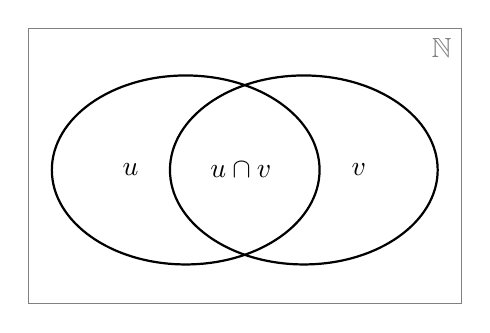
\begin{tikzpicture}
  % Rectangle representing N (lighter, not focus)
  \draw[gray, thin, opacity=1] (-1.5,-1.5) rectangle (4,2) 
        node[anchor=north east] {$\mathbb{N}$};

  % Set u (ellipse)
  \draw[thick] (0.5,0.2) ellipse (1.7cm and 1.2cm);
  \node at (-0.2,0.2) {$u$};

  % Set v (ellipse)
  \draw[thick] (2.0,0.2) ellipse (1.7cm and 1.2cm);
  \node at (2.7,0.2) {$v$};

  % Intersection label
  \node at (1.2,0.2) {$u \cap v$};
\end{tikzpicture}

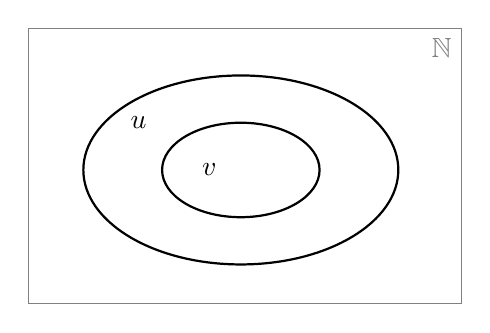
\begin{tikzpicture}
  % Rectangle for N (light, not focus)
  \draw[gray, thin, opacity=1] (-1.5,-1.5) rectangle (4,2) 
        node[anchor=north east] {$\mathbb{N}$};

  % Set u (outer ellipse)
  \draw[thick] (1.2,0.2) ellipse (2.0cm and 1.2cm);
  \node at (-0.1,0.8) {$u$};

  % Set v (nested inside)
  \draw[thick] (1.2,0.2) ellipse (1.0cm and 0.6cm);
  \node at (0.8,0.2) {$v$};
\end{tikzpicture}

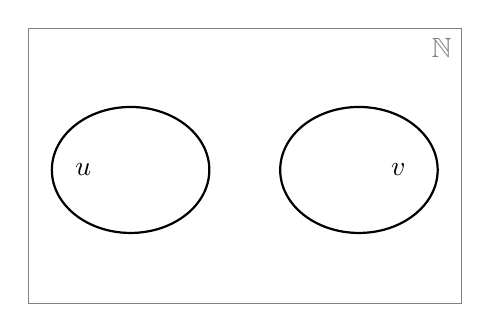
\begin{tikzpicture}
  % Rectangle for N (lighter, not focus)
  \draw[gray, thin, opacity=1] (-1.5,-1.5) rectangle (4,2)
        node[anchor=north east] {$\mathbb{N}$};

  % Set u (left, ellipse)
  \draw[thick] (-0.2,0.2) ellipse (1cm and 0.8cm);
  \node at (-0.8,0.2) {$u$};

  % Set v (right, ellipse, disjoint from u)
  \draw[thick] (2.7,0.2) ellipse (1cm and 0.8cm);
  \node at (3.2,0.2) {$v$};

  % Example index i inside v (optional)
  % \node at (2.5,-0.2) {$i$};
\end{tikzpicture}




\end{document}

